\documentclass[
%  draft,             % Testovací překlad
  12pt,               % Velikost základního písma je 12 bodů
  a4paper,            % Formát papíru je A4
%  oneside,           % Jednostranný tisk (výchozí)
% Z následujicich voleb lze použít maximálně jednu:
%    dvipdfm          % výstup bude zpracován programem 'dvipdfm' do PDF
%    dvips            % výstup bude zpracován programem 'dvips' do PS
%    pdftex           % překlad bude proveden programem 'pdftex' do PDF (výchozí)
    unicode,          % Záložky a informace budou v kódování unicode
% Z následujících voleb lze použít jen jednu:
%english,             % originální jazyk je angličtina
czech,                % originální jazyk je čeština (výchozí)
%slovak,              % originální jazyk je slovenčina
semestral             % semestrální práce
]{report}             % Dokument třídy 'zpráva'

\usepackage[utf8]     %    Kódování zdrojových souborů je v UTF-8
    {inputenc}        % Balíček pro nastavení kódování zdrojových souborů

\usepackage{graphicx} % Balíček 'graphicx' pro vkládání obrázků
                      % Nutné pro vložení log školy a fakulty

\usepackage[
    nohyperlinks      % Nebudou tvořeny hypertextové odkazy do seznamu zkratek
]{acronym}            % Balíček 'acronym' pro sazby zkratek a symbolů
                      % Nutné pro použití prostředí 'seznamzkratek' balíčku 'thesis'

\usepackage[
    breaklinks=true,    % Hypertextové odkazy mohou obsahovat zalomení řádku
    hypertexnames=false % Názvy hypertextových odkazů budou tvořeny
                        % nezávisle na názvech TeXu
]{hyperref}             % Balíček 'hyperref' pro sazbu hypertextových odkazů
                        % Nutné pro použití příkazu 'nastavenipdf' balíčku 'thesis'

\usepackage{pdfpages} % Balíček umožňující vkládat stránky z PDF souborů
                      % Nutné při vkládání titulních listů a zadání přímo
                      % ve formátu PDF z informačního systému

\usepackage{enumitem} % Balíček pro nastavení mezerování v odrážkách
  \setlist{topsep=0pt,partopsep=0pt,noitemsep}

\usepackage{cmap}     % Balíček cmap zajišťuje, že PDF vytvořené `pdflatexem' je
                      % plně "prohledávatelné" a "kopírovatelné"

\usepackage{upgreek}    % Balíček pro sazbu stojatých řeckých písmem
                        % např. stojaté pí: \uppi
                        % např. stojaté mí: \upmu (použitelné třeba v mikrometrech)
                        % pozor, grafická nekompatibilita s fonty typu Computer Modern!

\usepackage{dirtree}    % sazba adresářové struktury
\usepackage{amsmath}    % použití dfrac místo frac lepší zlomky
\usepackage{float}      % H aby obrázky a tabulky neuplavali
\usepackage{pdflscape}  % otočení pdf na šířku
\usepackage{pdfpages}   % vložení pdf stránky


\usepackage{tikz}
\usetikzlibrary{automata, positioning, arrows, shapes}

%%TIKZ style

% Define block styles
\tikzstyle{decision} = [diamond, draw,text width=7em, text badly centered, node distance=3cm, inner sep=0pt, aspect=2]
\tikzstyle{block} = [rectangle, draw, text width=3cm, text centered, rounded corners, minimum height=2em]
\tikzstyle{line} = [draw, -latex']
\tikzstyle{round} = [draw, ellipse, node distance=3cm, minimum height=2em]
\tikzstyle{subroutine} = [draw, rectangle split, rectangle split horizontal, rectangle split parts=3]

\usepackage[formats]{listings} % Balíček pro sazbu zdrojových textů

\usepackage{color}

\definecolor{codegreen}{rgb}{0,0.6,0}
\definecolor{codegray}{rgb}{0.5,0.5,0.5}
\definecolor{codepurple}{rgb}{0.58,0,0.82}
\definecolor{backcolour}{rgb}{0.95,0.95,0.92}

\lstdefinestyle{mystyle}{
    backgroundcolor=\color{backcolour},
    commentstyle=\color{codegreen},
    keywordstyle=\color{magenta},
    numberstyle=\tiny\color{codegray},
    stringstyle=\color{codepurple},
    basicstyle=\footnotesize,
    breakatwhitespace=false,
    breaklines=true,
    captionpos=b,
    keepspaces=true,
    numbers=left,
    numbersep=5pt,
    showspaces=false,
    showstringspaces=false,
    showtabs=false,
    tabsize=2
}

\lstset{style=mystyle}

\lstset{
language=C++,                	  % choose the language of the code
numbers=left,                   % where to put the line-numbers
stepnumber=1,                   % the step between two line-numbers.
numbersep=5pt,                  % how far the line-numbers are from the code
backgroundcolor=\color{backcolour},  % choose the background color. You must add \usepackage{color}
showspaces=false,               % show spaces adding particular underscores
showstringspaces=false,         % underline spaces within strings
showtabs=false,                 % show tabs within strings adding particular underscores
tabsize=2,                      % sets default tabsize to 2 spaces
captionpos=b,                   % sets the caption-position to bottom
breaklines=true,                % sets automatic line breaking
breakatwhitespace=true,         % sets if automatic breaks should only happen at whitespace
%title=~%firmware kostky 08.12.2016,                 % show the filename of files included with \lstinputlisting;
%    Definice jazyka použitého ve výpisech
%    language=[LaTeX]{TeX},    % LaTeX
%    language={Matlab},        % Matlab
    inputencoding=utf8,        % pro soubory uložené v kódování UTF-8
    %inputencoding=cp1250,     % pro soubory uložené ve standardním kódování Windows CP1250
%        columns=fixed,         %flexible,
%        fontadjust=true        %licovani sloupcu
    extendedchars=true,
    literate=                  % definice symbolů s diakritikou
    {á}{{\'a}}1
    {č}{{\v{c}}}1
    {ď}{{\v{d}}}1
    {é}{{\'e}}1
    {ě}{{\v{e}}}1
    {í}{{\'i}}1
    {ň}{{\v{n}}}1
    {ó}{{\'o}}1
    {ř}{{\v{r}}}1
    {š}{{\v{s}}}1
    {ť}{{\v{t}}}1
    {ú}{{\'u}}1
    {ů}{{\r{u}}}1
    {ý}{{\'y}}1
    {ž}{{\v{z}}}1
    {Á}{{\'A}}1
    {Č}{{\v{C}}}1
    {Ď}{{\v{D}}}1
    {É}{{\'E}}1
    {Ě}{{\v{E}}}1
    {Í}{{\'I}}1
    {Ň}{{\v{N}}}1
    {Ó}{{\'O}}1
    {Ř}{{\v{R}}}1
    {Š}{{\v{S}}}1
    {Ť}{{\v{T}}}1
    {Ú}{{\'U}}1
    {Ů}{{\r{U}}}1
    {Ý}{{\'Y}}1
    {Ž}{{\v{Z}}}1
}


% Nastavení českého jazyka při sazbě v češtině.
\usepackage
  {babel}                 % Balíček pro sazbu různojazyčných dokumentů; kompilovat (pdf)latexem!
                          % převezme si z parametrů třídy správný jazyk
\usepackage{lmodern}      % vektorové fonty Latin Modern, nástupce půvoních Knuthových Computern Modern fontů
\usepackage{textcomp}     % Dodatečné symboly
\usepackage[T1]{fontenc}  % Kódování fontu - mj. kvůli správným vzorům pro dělení slov
\usepackage[bf]{caption2} % změna fontu

\usepackage[%
% Z následujících voleb lze použít pouze jednu
% left,                   % Rovnice a popisky plovoucich objektů budou %zarovnány vlevo
  center,                 % Rovnice a popisky plovoucich objektů budou zarovnány na střed (vychozi)
% Z následujících voleb lze použít pouze jednu
semestral                 % sazba zprávy semestrálního projektu
%bachelor                 % sazba bakalářské práce
%diploma                  % sazba diplomové práce
%treatise                 % sazba pojednání o dizertační práci
%phd                      % sazba dizertační práce
]{book/style/thesis}      % Balíček pro sazbu studentských prací
                          % Musí být vložen až jako poslední, aby
                          % ostatní balíčky nepřepisovaly jeho příkazy

%%%%%%%%%%%%%%%%%%%%%%%%%%%%%%%%%%%%%%%%%%%%%%%%%%%%%%%%%%%%%%%%%
%%%%%%      Definice informací o dokumentu             %%%%%%%%%%
%%%%%%%%%%%%%%%%%%%%%%%%%%%%%%%%%%%%%%%%%%%%%%%%%%%%%%%%%%%%%%%%%

\input{book/sablony-nastav_udaju} % do tohoto souboru doplňte údaje o sobě, o názvu práce...

%%%%%%%%%%%%%%%%%%%%%%%%%%%%%%%%%%%%%%%%%%%%%%%%%%%%%%%%%%%%%%%%%%%%%%%%

%%%%%%%%%%%%%%%%%%%%%%%%%%%%%%%%%%%%%%%%%%%%%%%%%%%%%%%%%%%%%%%%%%%%%%%%
%%%%%%     Nastavení polí ve Vlastnostech dokumentu PDF      %%%%%%%%%%%
%%%%%%%%%%%%%%%%%%%%%%%%%%%%%%%%%%%%%%%%%%%%%%%%%%%%%%%%%%%%%%%%%%%%%%%%
%% Při vloženém balíčku 'hyperref' lze použít příkaz '\nastavenipdf'
\nastavenipdf
%  Nastavení polí je možné provést také ručně příkazem:
%\hypersetup{
%  pdftitle={Název studentské práce},        % Pole 'Document Title'
%  pdfauthor={Autor studenstké práce},       % Pole 'Author'
%  pdfsubject={Typ práce},                   % Pole 'Subject'
%  pdfkeywords={Klíčová slova}               % Pole 'Keywords'
%}
%%%%%%%%%%%%%%%%%%%%%%%%%%%%%%%%%%%%%%%%%%%%%%%%%%%%%%%%%%%%%%%%%%%%%%%

%%%%%%%%%%%%%%%%%%%%%%%%%%%%%%%%%%%%%%%%%%%%%%%%%%%%%%%%%%%%%%%%%%%%%%%
%%%%%%%%%%%       Začátek dokumentu               %%%%%%%%%%%%%%%%%%%%%
%%%%%%%%%%%%%%%%%%%%%%%%%%%%%%%%%%%%%%%%%%%%%%%%%%%%%%%%%%%%%%%%%%%%%%%
\begin{document}


% Vložení desek generovaných informačním systémem
\includepdf[pages=1,offset=15.4mm -1in]%
  {book/pdf/student-desky} % název souboru nesmí obsahovat mezery!
% nebo vytvoření desek z balíčku
%\vytvorobalku
\setcounter{page}{1} %resetovani citace stranek - desky se necisluji

%% Vložení titulního listu generovaného informačním systémem
\includepdf[pages=1,offset=15.4mm -1in]%
  {book/pdf/student-titulka}% název souboru nesmí obsahovat mezery!
% nebo vytvoření titulní stránky z balíčku
%\vytvortitulku

% Vložení zadání generovaného informačním systémem
\includepdf[pages=1,offset=15.4mm -1in]%
  {book/pdf/student-zadani}% název souboru nesmí obsahovat mezery!
% nebo lze vytvořit prázdný list příkazem ze šablony
%\stranka{}%
%    {\sffamily\Huge\centering ZDE VLOŽIT LIST ZADÁNÍ}%
%    {\sffamily\centering Z~důvodu správného číslování stránek}

% Vysázení stránky s abstraktem
\vytvorabstrakt

% Vysázení prohlaseni o samostatnosti
\vytvorprohlaseni

% Vysázení poděkování
\vytvorpodekovani

% Vysázení poděkování projektu SIX
% zakomentujte pokud neodpovida realite
%\vytvorpodekovaniSIX

% Vysázení obsahu
\obsah

% Vysázení seznamu obrázků
\seznamobrazku

% Vysázení seznamu tabulek
\seznamtabulek

% Vysázení seznamu výpisů
% \lstlistoflistings

% Vložení souboru 'text/uvod.tex' s úvodem
\chapter*{Úvod}
\phantomsection
\addcontentsline{toc}{chapter}{Úvod}

bližší rozbor a diskuze zadání, jeho upřesnění a doplnění, konkretizace cílů práce


% Vložení souboru 'text/reseni' s popisem reseni práce
\chapter[Teoretická část studentské práce]{Teoretická část studentské\\ práce}

%\section{Laser Game}

\zkratka{LG}, někdy také nazývána i Laser Tag, je označení pro společenské hry, motivované sci-fi, využívající moderní elektroniku. Hráči získávají body za zásahy \zkratka{IR} paprskem z jejich zbraně do zásahových čidel soupeřů, či jiných objektů zásahovým čidlem vybaveným. A naopak o své body přicházejí, pokud se jejich zásahová čidla stanou terčem nepřátelských \zkratka{IR} paprsků.

Nejčasteji se hra odehrává v místnosi speciálně upravené pro tento účel, označované jako aréna. Stěny, strop a podlaha arény bývají zpravidla pokryty tmavou barvou (černé koberce, koženky a podobné materiály) tak, aby se zabránilo odrazům \zkratka{IR} paprsků. Zdi v arénách jsou často vypolstrovány, aby se snížilo riziko zranění hráčů. Obvykle arény nejsou jen klasické místnosti se čtyřmi stěnami a rovnou podlahou, nýbrž často bývají značně členité, vybavené úkryty a překážkami.

Pro zpestření hry mohou být arény vybaveny i další elektornikou, například optickými závorami, minami či světělnými a kouřovými efekty.

\section{Úvod do problematiky Laser Game systému}

\subsection{Laser Game}
\zkratka{LG}, někdy také nazývána i Laser Tag, je označení pro společenské hry, motivované sci-fi, využívající moderní elektroniku. Hráči získávají body za zásahy \zkratka{IR} paprskem z jejich zbraně do zásahových čidel soupeřů, či jiných objektů zásahovým čidlem vybaveným. A naopak o své body přicházejí, pokud se jejich zásahová čidla stanou terčem nepřátelských \zkratka{IR} paprsků. Cílem každého hráče je zíshat co nejvíce bodů.

Nejčasteji se hra odehrává v místnosi speciálně upravené pro tento účel, označované jako aréna. Stěny, strop a podlaha arény bývají zpravidla pokryty tmavou barvou (černé koberce, koženky a podobné materiály) tak, aby se zabránilo odrazům \zkratka{IR} paprsků. Zdi v arénách jsou často vypolstrovány, aby se snížilo riziko zranění hráčů. Obvykle arény nejsou jen klasické místnosti se čtyřmi stěnami a rovnou podlahou, nýbrž často bývají značně členité, vybavené úkryty a překážkami.

Pro zpestření hry mohou být arény vybaveny i další elektornikou, například optickými závorami, minami či světělnými a kouřovými efekty.



\subsection{Historie Laser Game}
Koncem sedmdesátých a na začátku osmdesátách let vyvýjela firma Lockheed Martin Information Systems pro armádu spojených států amerických systém, využívající \zkratka{IR} paprsky pro tréning boje navývaný \zkratka{MILIES}. Systém funguje na stjeném principu jako \zkratka{LG}. Voják má na hlavni zbraně \zkratka{IR} vysílač. Ten reaguje na stisk spoutě. Voják je oděn ve speciálním obleku z \zkratka{IR} senzory. Při zásahu vojáka jsou odeslány z obleku informace do řídící jednotky, která vyhodtí, jestli je voják zraněný a nebo mrtev. Používání tohoto systému je bezpečnější než využívání konvenčních zbraní. V roce 1992 vyšla nová verze tohoto systému pojmenovaná MILIES2000, který navíc po zabití vojáka zablokuje jeho další střelbu a akusticky ohlásí zasažení. \zkratka{MILIES} využívá od roku 2002 i armáda žeské rebubliky a  také i ostatní země \zkratka{NATO}.

Prvním komerčne prodávaným zařízneím, se který je spojován vznik \zkratka{LG} je hračka Star Trek Electronic Phaser od společnosti South end Electronics, která byla uvedena na trh v roce 1979. Hračka má tvar futuristické zbraně inspirované Star Trekem. Součástí zbraně je signalizační blok, který pomocí \zkratka{LED} a reproduktoru indikuje zásah a \zkratka{IR} vysílač pro palbu.
\footnote{\url{https://en.wikipedia.org/wiki/Laser_tag} [cit. 21.11.2017]}

\subsection{Laser Game systém}
\zkratka{LG} systém je soustava zahrnující \zkratka{HW}, \zkratka{FW} a \zkratka{SW} umožnující hrát \zkratka{LG}. \zkratka{LG} systém lze tedy chápat jako vybavení nezbytné pro provozování \zkratka{LG} arény.

Nejdůležitějšími součástmi \zkratka{LG} systému jsou vesty, zbraně, kominikační router a řídící \zkratka{PC}, \zkratka{LG} systém může být dále doplněn například o optické závory, miny či bomby.

\subsection{Řídící počítač}
Řídící počítač má za úkol prostřednictvím routru komunikovat s vestami, případně i dalšími zařízeními v síti. Hostuje řídící \zkratka{SW}, pomocí nehož operátor arény ovládá hru. Zajišťuje nakonfigurování vest. V průběhu hry stahuje z vest údaje a vyhodnocuje pořadí hráčů.

\subsection{Router}
Zajišťuje směrování v bezdrátové \zkratka{LG} síti. Sprostředkovává tedy duplexní spojení mezi vestami a počítačem.

\subsection{Vesta}
Vesta je oděv který nosí hráči \zkratka{LG}. Má dvě hlavní funkce, detekovat zásahy a komunikovat s řídícím počítačem. Další funkcí vesty je barevná identifikace hráčů pomocí \zkratka{RGB} \zkratka{LED}. Vesta může zajišťovat i zvukové efekty, zobrazovat hráči jeho statistiky z aktuální hry. Vesta také komunikuje s hráčovou zbraní.

\subsection{Zbraň}
Zbraň má jednoduchou úlohu, zajištuje vysílání \zkratka{IR} paprsku, který při zásahu vesty zabije hráče (jde o zabité ve hře ne o skutečné usmrcení).

\subsection{Laser Game systémy na trhu}



% Vložení souboru 'text/vysledky' s popisem vysledků práce
\include{book/text/vysledky}

% Vložení souboru 'text/zaver' se závěrem
\chapter{Závěr}

Podařilo se mi navrhnout velmi spolehlivý protokol pro přenos dat pomocí infračerveného záření, založený na 16\jedn{b} CRC, díky tomu je chybovost systému $1,526 \cdot 10^{-5}$. První verze návrhu se potýkala s problémem zahlcování detektorů shluky nul a následnou chybnou interpretací zkreslených dat.

Druhá verze problémy odstranila návrhem nového robustního komunikačního protokolu. Navržený protokol korektně přenáší i rámce plné nul, protože byla změněna reprezentace logických hodnot v komunikaci ze stavů svítí nesvítí na pulzy definovaných délek. Výhodou tohoto systému je i možnost zjistit výpadek při probíhající komunikaci, protože i nula je přenášena jako pulz.

Dále byl navržený komunikační protokol pro rádiovou komunikaci v hvězdicové síti, který je založený na rámcích proměnných délek, schopný v jednom rámci pojmout až 512~\jedn{B} dat. Protokol k ověřování platnosti dat používá 32\jedn{b} CRC, takže pravděpodobnost chyby je prakticky nulová ($2,328 \cdot 10^{-10}$).

V průběhu práce byla zhotovena a oživena elektronika pro dvě vesty a komunikační router. Cenové náklady na součástky a plošné spoje na jednu vestu se pohybují okolo 4 000~\jedn{Kč}, do nákladů ale není zahrnutý čas strávený vývojem a také není uvažována cena krabiček. V porovnání s cenami systému EVO-5, kde v přepočtu cena jedné vesty při koupi 16 vest se pohybuje okolo 50 000~\jedn{Kč} je vybavení arény mím systémem mnohem levnější.

Výsledky mé práce jsou dostupné na mém \href{https://github.com/wykys}{osobním githubu}, případně na \href{https://github.com/laser-game}{githubu organizace laser geme}.  


% Vložení souboru 'text/literatura' se seznamem literatury
\begin{literatura}{99}

\bibitem{senzory}
    MARTINEK, Radislav.
    \emph{Senzory v průmyslové praxi.}
    Praha: BEN - technická literatura, 2004. ISBN 80-7300-114-4.

\bibitem{elektronika}
    FROHN, Manfred.
    \emph{Elektronika: polovodičové součástky a základní zapojení}
    Praha: BEN - technická literatura, 2006. ISBN 80-7300-123-3.

\end{literatura}


% Vložení souboru 'text/zkratky' se seznam použitých symbolů, veličin a zkratek
\begin{seznamzkratek}{KolikMista}

    \novazkratka{IR}
        {IR}
        {infra červený -- Infra Red}

    \novazkratka{RGB}
        {RGB}
        {červená-zelená-modrá -- Red Green Blue}

    \novazkratka{LED}
        {LED}
        {světlo emitující dioda -- Light Emitting Diode}

    \novazkratka{LG}
        {LG}
        {Laser Game}

    \novazkratka{SW}
        {SW}
        {Software}

    \novazkratka{FW}
        {FW}
        {Firmware}

    \novazkratka{HW}
        {HW}
        {Hardware}

    \novazkratka{PC}
        {PC}
        {osobní počítač -- Personal Computer}

    \novazkratka{MILIES}
        {MILIES}
        {vojenský simulátor střelby -- Multiple Integrated Laser Engagement System}

    \novazkratka{NATO}
        {NATO}
        {Severoatlantická aliance -- North Atlantic Treaty Organization}

    \novazkratka{DPS}
        {DPS}
        {Deska Plošných Spojů}

    \novazkratka{symfvz}
        {\ensuremath{f_\textind{vz}}}
        {vzorkovací kmitočet}

\end{seznamzkratek}


% Začátek příloh
\prilohy

% Vysázení seznamu příloh
%\seznampriloh

% Vložení souboru 'text/prilohy' s přílohami
\chapter*{Přiložená schémata zapojení}

%\begin{landscape}
    %    \begin{figure}[h]
    %	    \centering
    %	    \includegraphics[height=\textwidth]{sch/main_board_part_a}
    %	    \caption{Schéma zapojení hlavní desky vesty první část}
    %    \end{figure}
    %\end{landscape}
    %
    %\begin{landscape}
    %    \begin{figure}[h]
    %	    \centering
    %	    \includegraphics[height=\textwidth]{sch/main_board_part_b}
    %	    \caption{Schéma zapojení hlavní desky vesty druhá část}
    %    \end{figure}
    %\end{landscape}
    %
    %\begin{landscape}
    %    \begin{figure}[h]
    %	    \centering
    %	    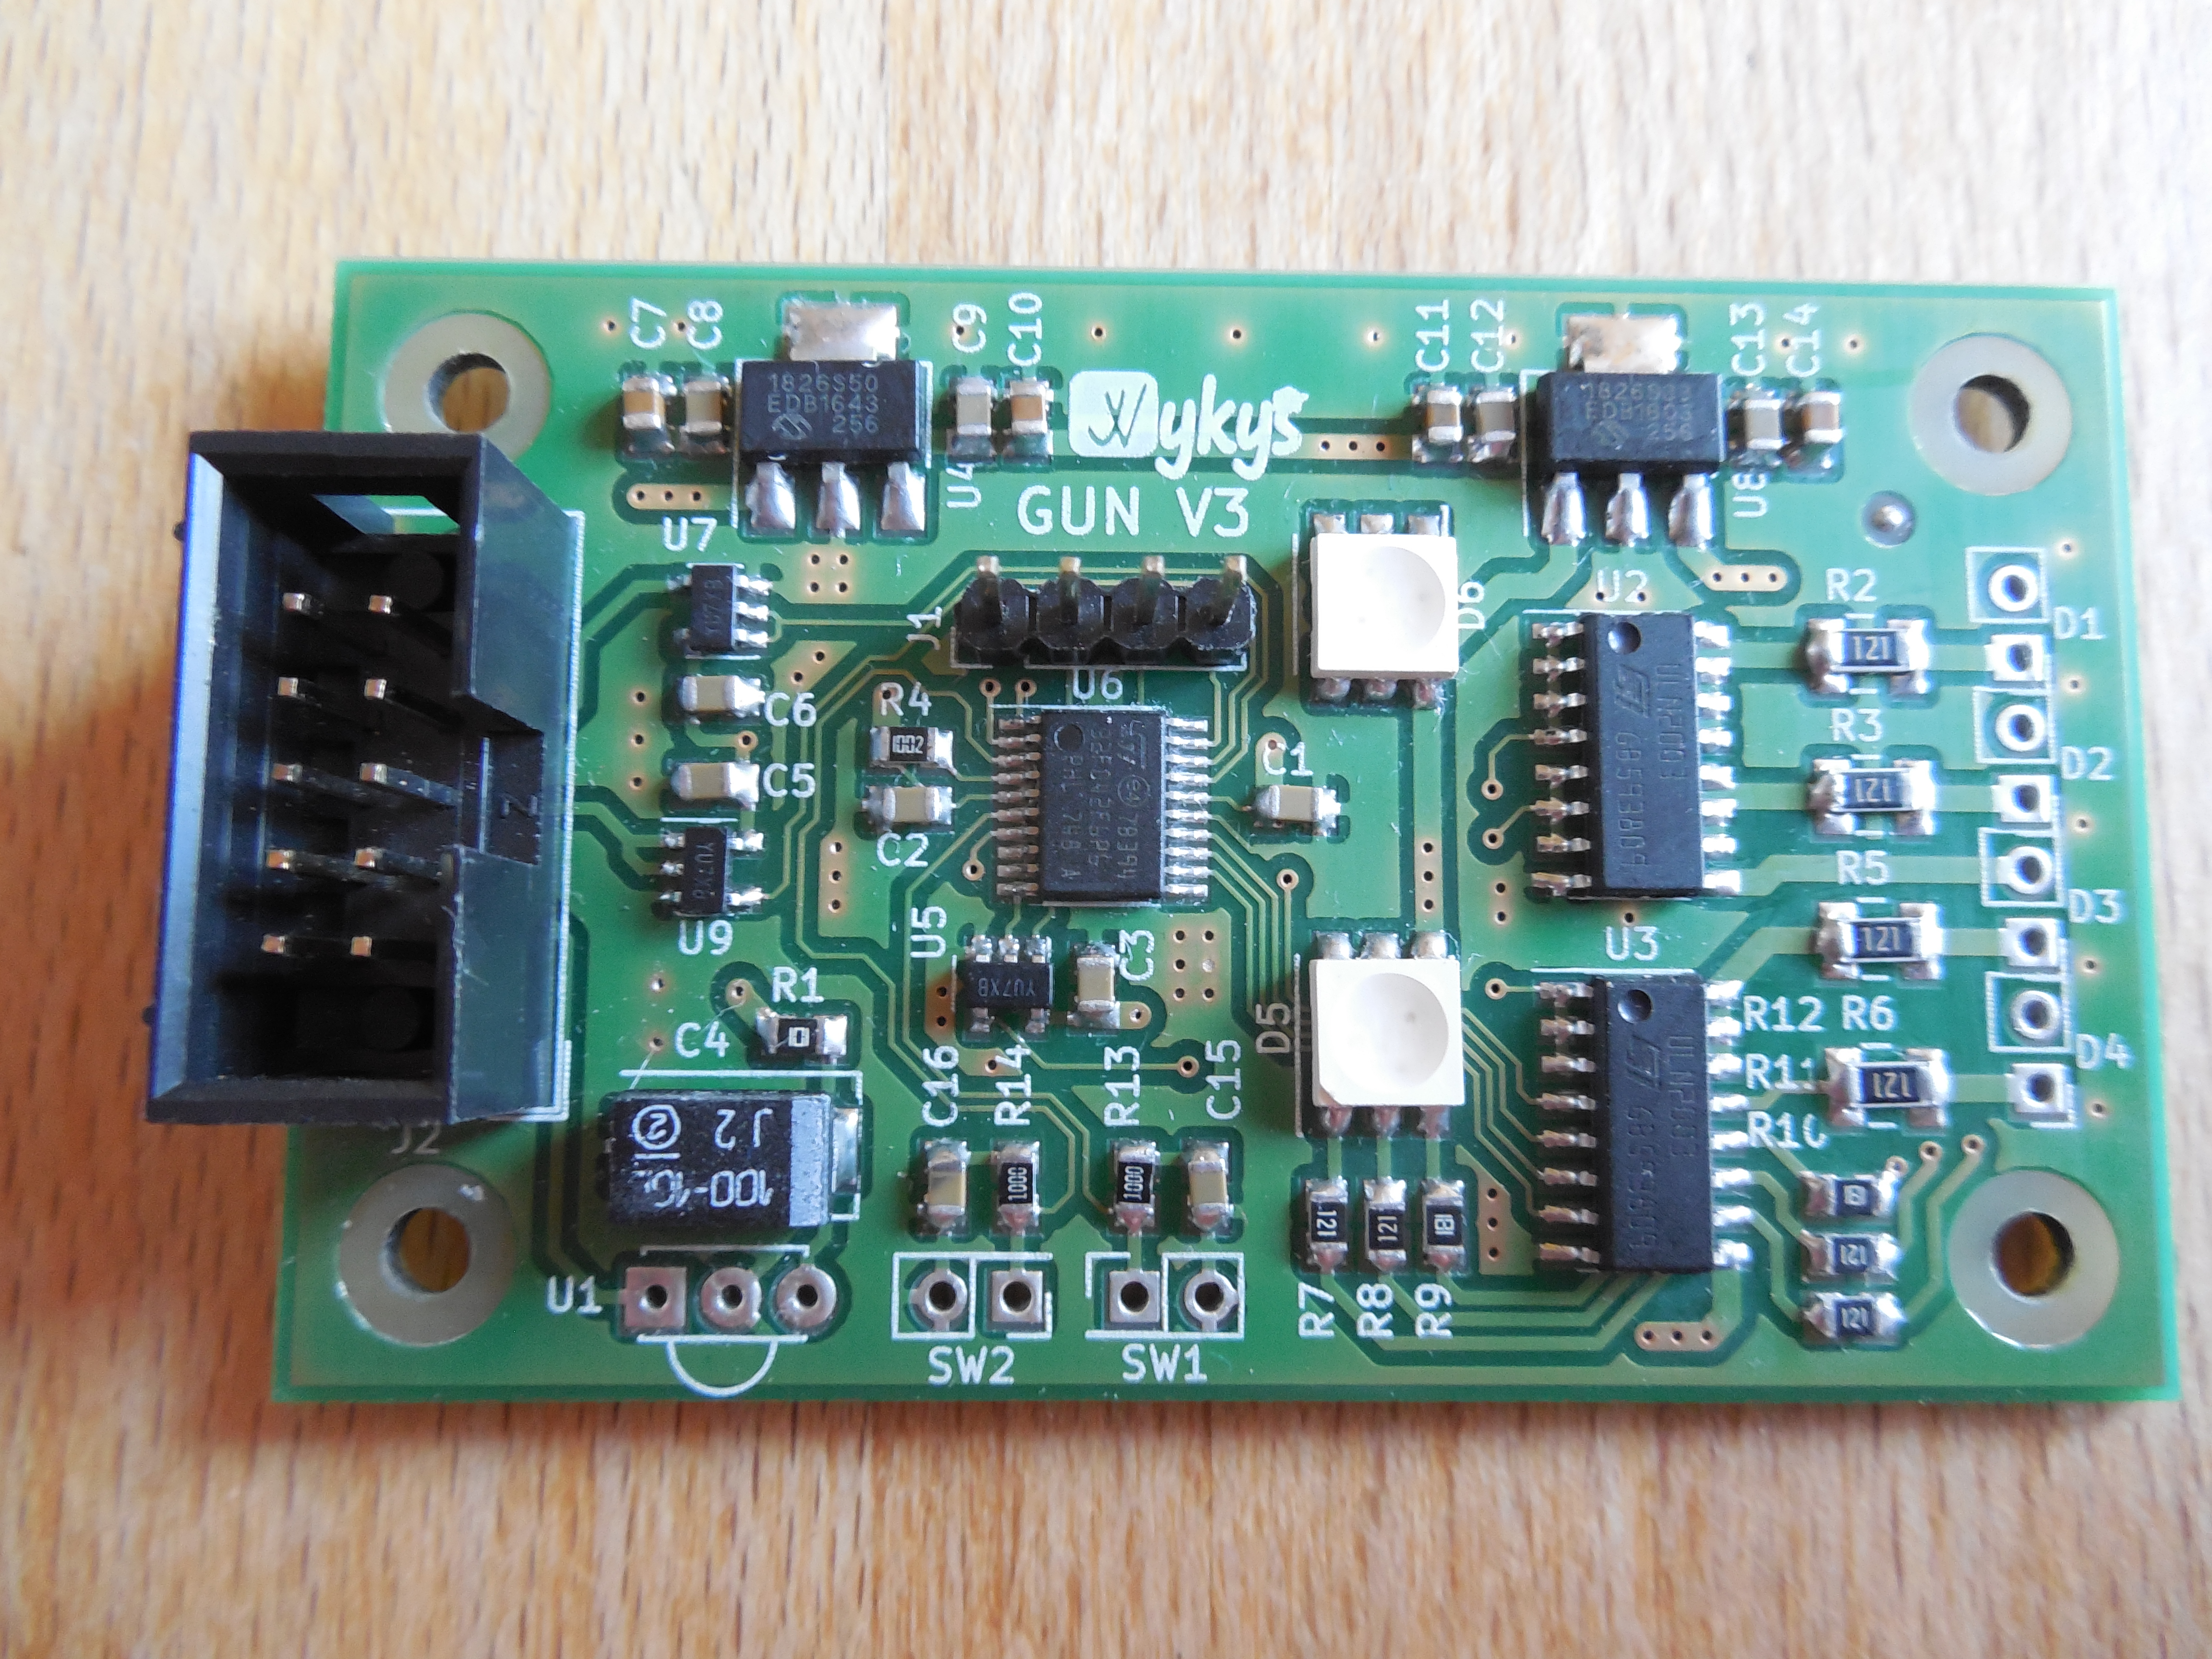
\includegraphics[height=\textwidth]{sch/gun}
    %	    \caption{Schéma zapojení zbraně}
    %    \end{figure}
    %\end{landscape}
    %
    %\begin{landscape}
    %    \begin{figure}[h]
    %	    \centering
    %	    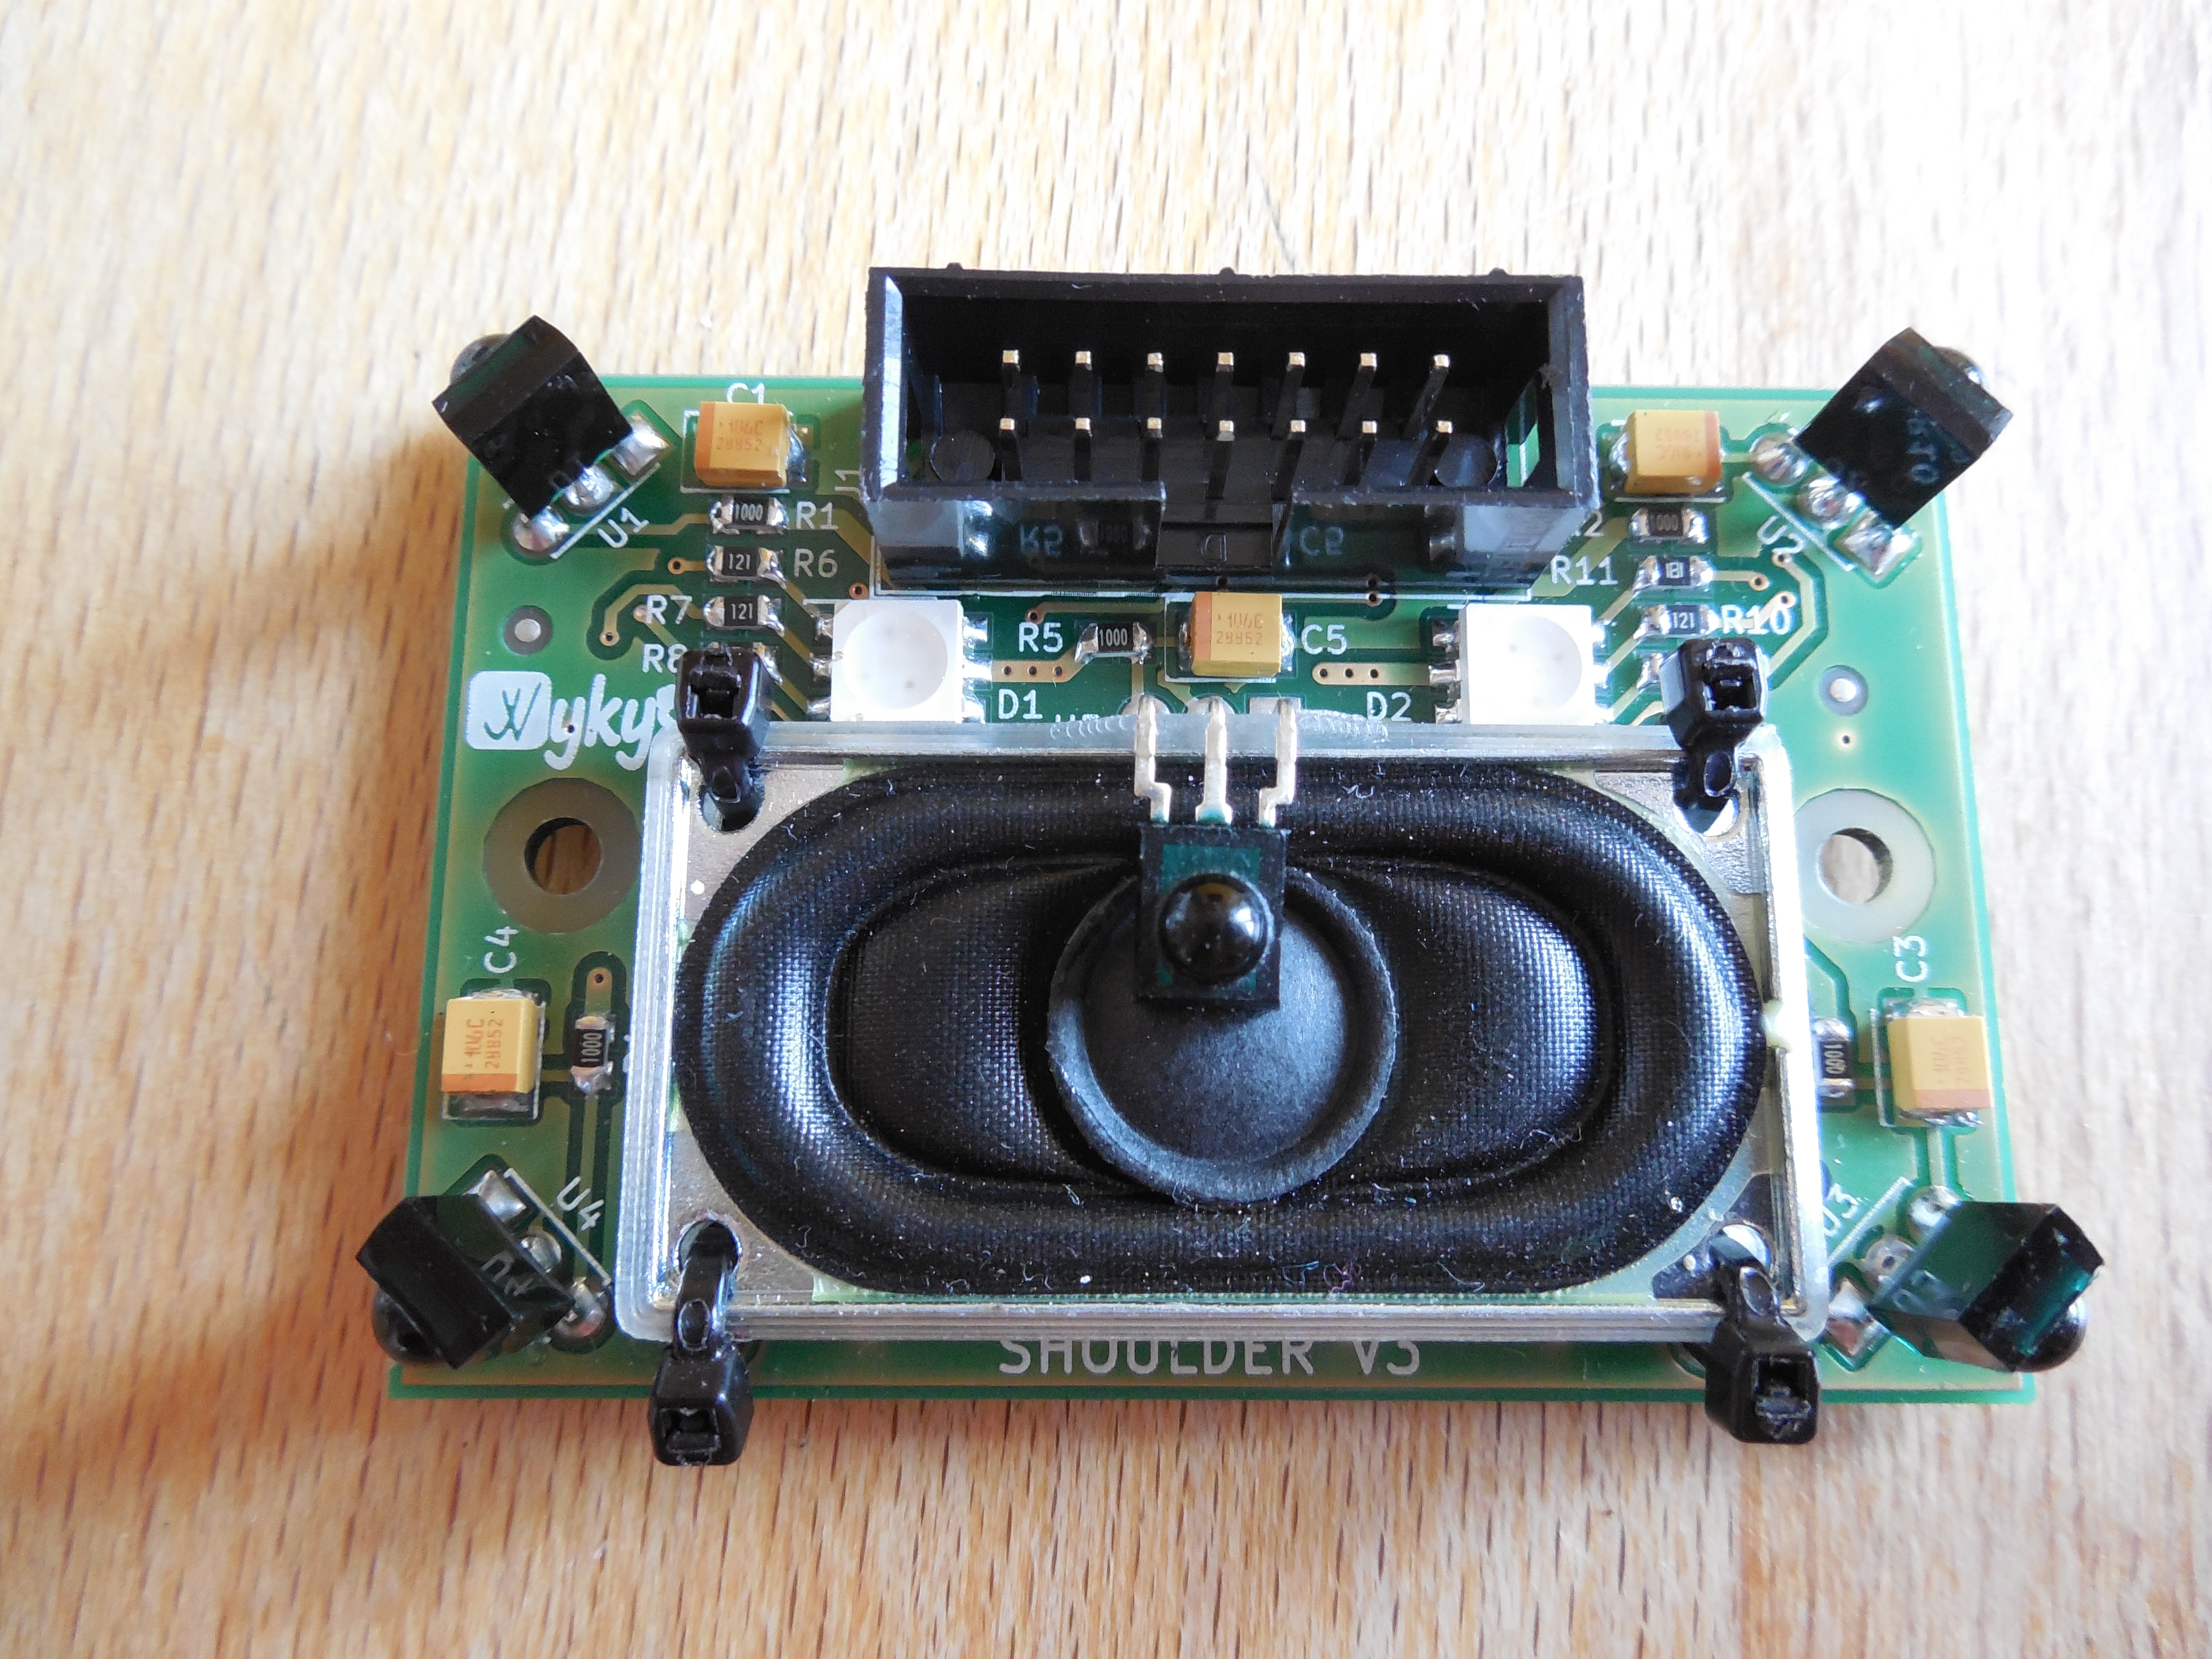
\includegraphics[height=\textwidth]{sch/shoulder}
    %	    \caption{Schéma zapojení ramene}
    %    \end{figure}
    %\end{landscape}
    %
    %\begin{landscape}
    %    \begin{figure}[h]
    %	    \centering
    %	    \includegraphics[height=\textwidth]{sch/display_board}
    %	    \caption{Schéma zapojení znakového terminálu}
    %    \end{figure}
    %\end{landscape}
    %
    %\begin{landscape}
    %    \begin{figure}[h]
    %	    \centering
    %	    \includegraphics[height=\textwidth]{sch/wireless_box}
    %	    \caption{Schéma zapojení rádiové komunikace}
    %    \end{figure}
    %\end{landscape}
    %
    %\begin{landscape}
    %    \begin{figure}[h]
    %	    \centering
    %	    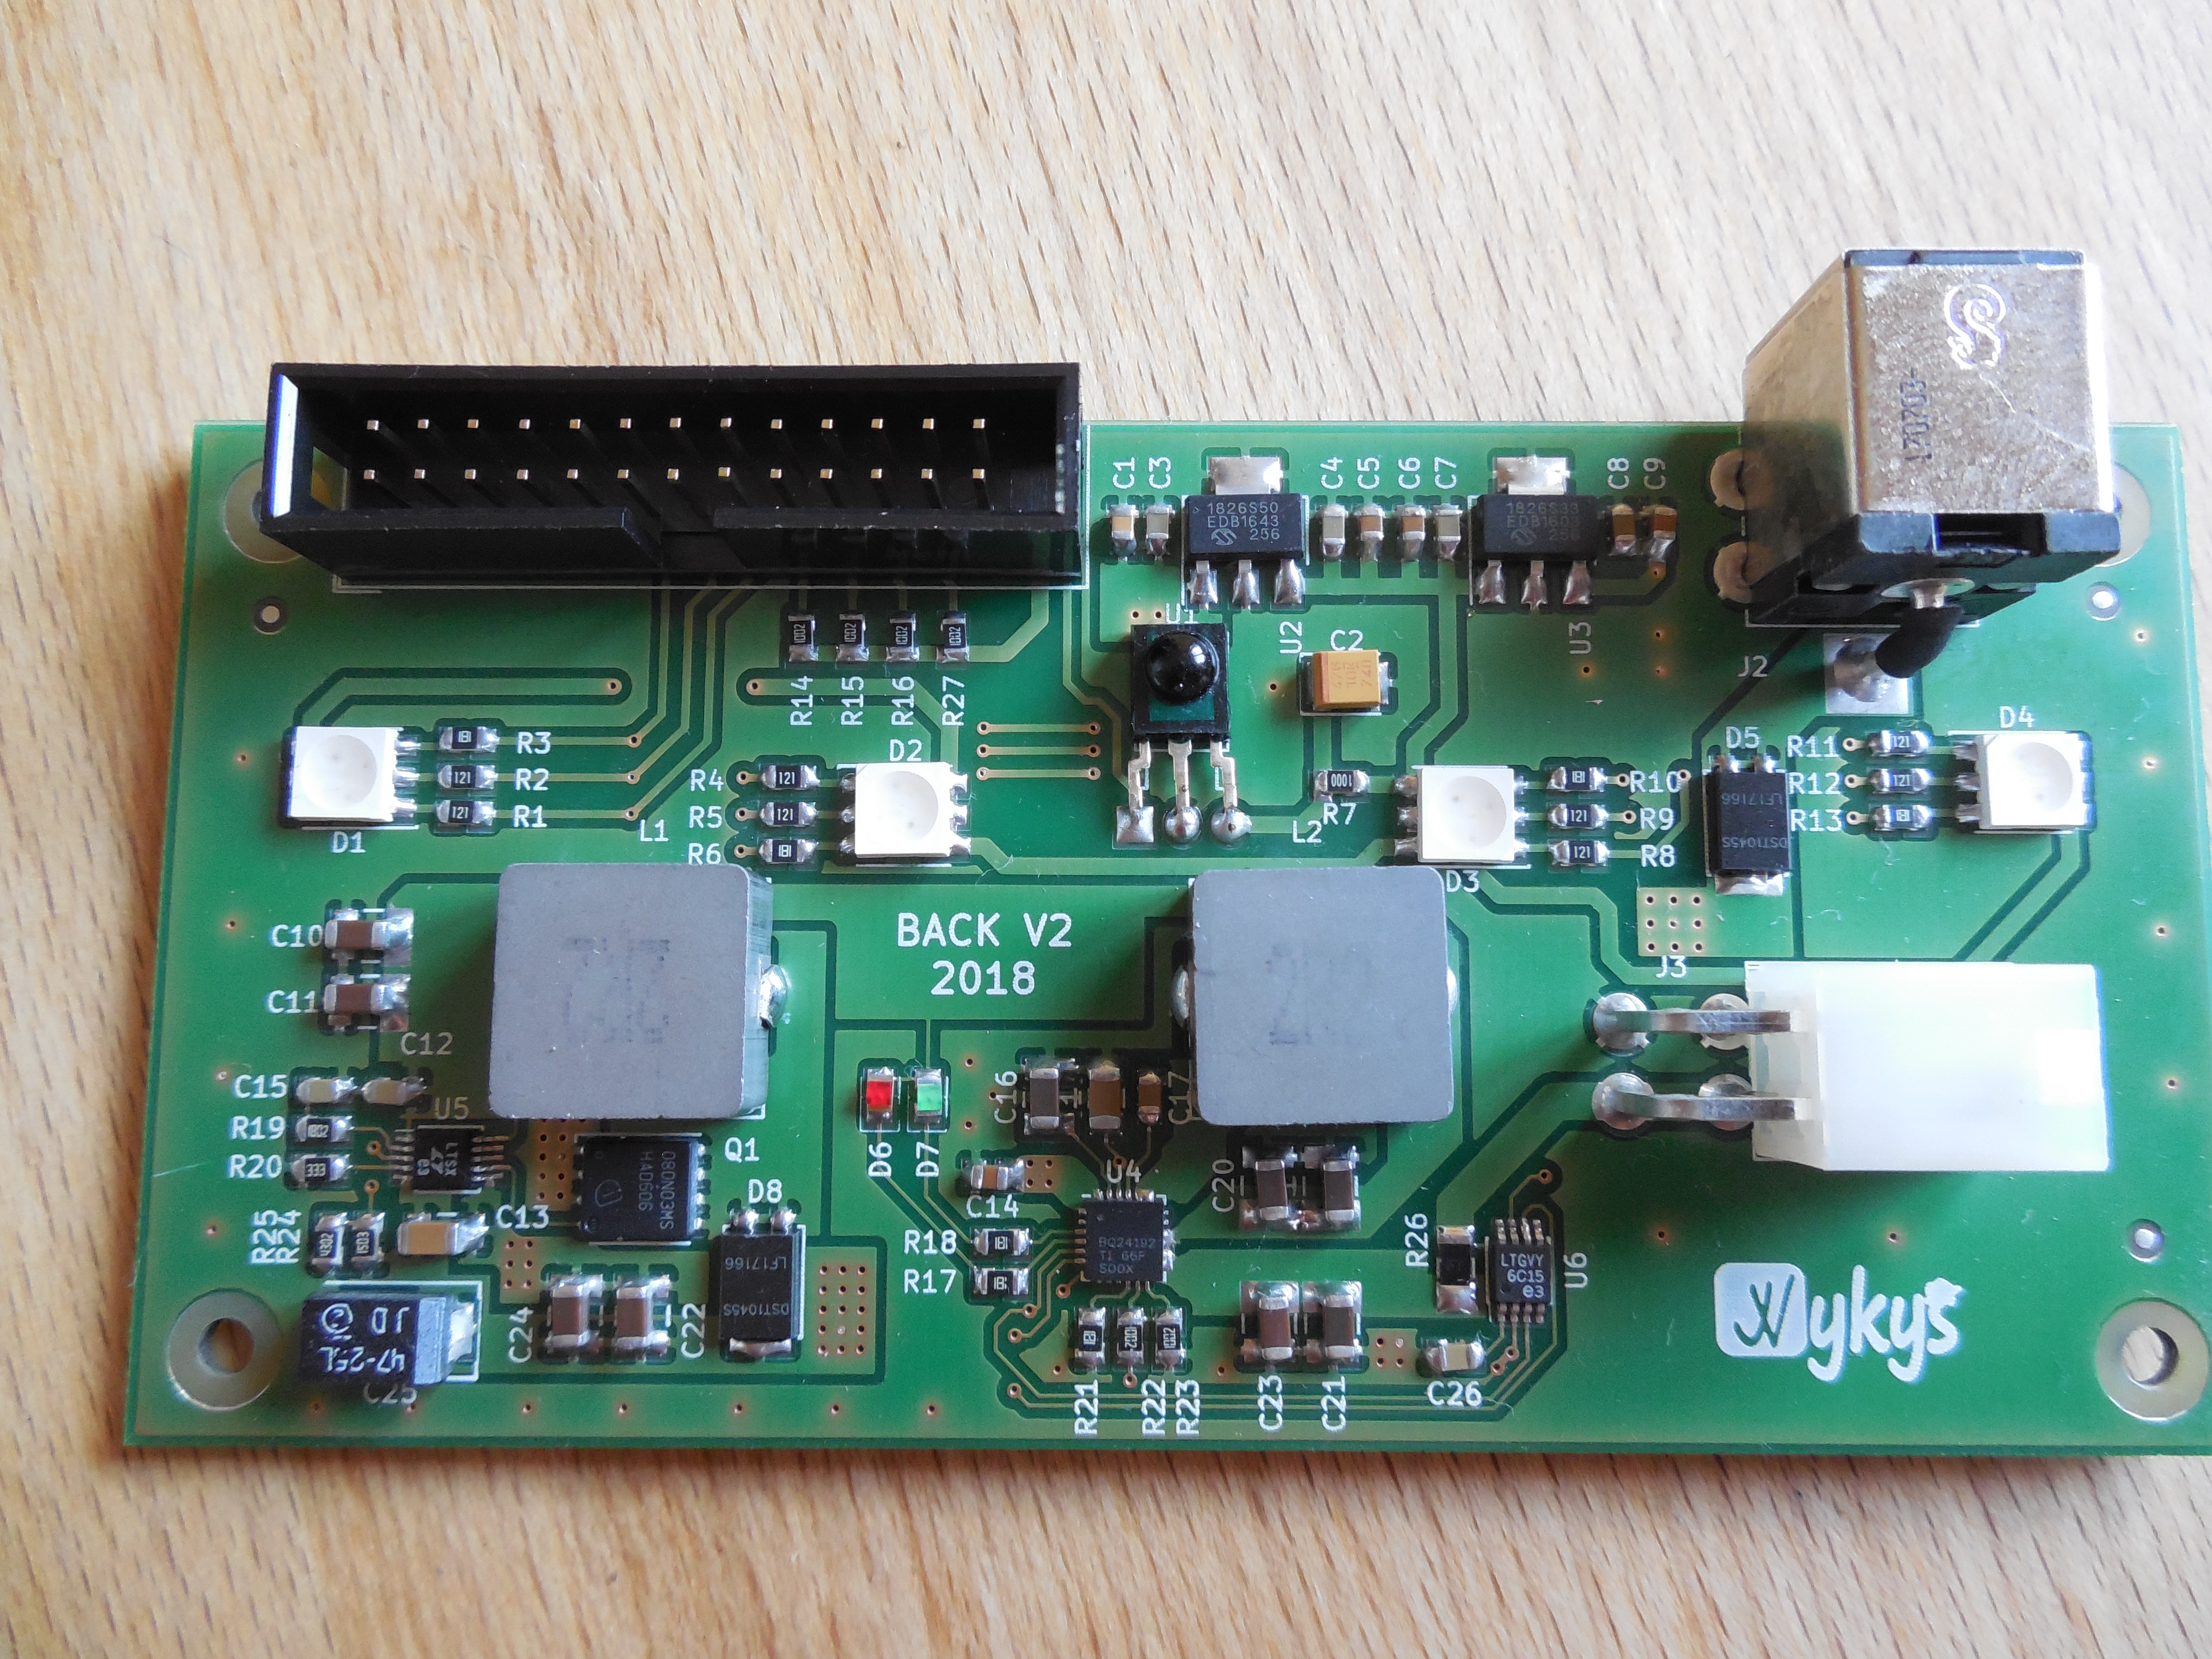
\includegraphics[height=\textwidth]{sch/back}
    %	    \caption{Schéma zapojení desky na záda s integrovanou nabíječkou}
    %    \end{figure}
    %\end{landscape}


% Konec dokumentu
\end{document}
